\documentclass[a4paper,10pt]{article}
\usepackage{hyperref}
\usepackage{graphicx}
\usepackage{url}
\usepackage{lmodern}
\usepackage[T1]{fontenc}
\usepackage{listings}


% Title Page
\title{Historical Conflict Abstractization using NLP}
\author{Carcu Bogdan}


\begin{document}
\maketitle

\tableofcontents
\section{Overview}

 \subsection{Running instructions}
 You can choose your OS, Python version and language model.
 For this tutorial, Windows, Python 3.x and English were chosen

 Write in the command line:
 "python -m pip install -U spacy
  python -m spacy download en"

  For more guidance, visit https://spacy.io/usage

  Create a file with the extension ".py"
  Import spacy: write "import spacy"

  Create a Doc object and call nlp function on the required text/file.
 \begin{lstlisting}[language=Python]
  Test:

  doc = nlp(u'Apple is looking at buying U.K. startup for 1 billion')

  for token in doc:
    print(token.text, token.lemma_, token.pos_, token.tag_, token.dep_,
          token.shape_, token.is_alpha, token.is_stop)

 \end{lstlisting}
  The text is tokanized automatically by creating the Doc object.
  Run it. Now you are ready to go!
 
 \subsection{Theoretical aspects}

  \quad Processing raw text intelligently is difficult: most words are rare, and it's common for words that look completely different to mean almost the same thing. The same words in a different order can mean something completely different. Even splitting text into useful word-like units can be difficult in many languages.
  \newline During processing, first tokenize the text, i.e. segments it into words, punctuation and so on. This is done by applying rules specific to each language. For example, punctuation at the end of a sentence should be split off, whereas "U.K." should remain one token.
  \newline First, the raw text is split on whitespace characters, similar to text.split(' ') in Python. Then, the tokenizer processes the text from left to right. On each substring, it performs two checks:
   \begin{itemize}
  \item Does the substring match a tokenizer exception rule? For example, "don't" does not contain whitespace, but should be split into two tokens, "do" and "n't", while "U.K." should always remain one token.
  \item Can a prefix, suffix or infix be split off? For example, punctuation like commas, periods, hyphens or quotes.
  If there's a match, the rule is applied, and the tokenizer continues its loop, starting with the newly split substrings.
   \end{itemize}

  Tokenization is the task of splitting a text into meaningful segments, called tokens.
  How? \newline
  \begin{itemize}
  \item During processing, first tokenize the text, i.e. segments it into words, punctuation and so on. This is done by applying rules specific to each language. For example, punctuation at the end of a sentence should be split off, whereas "U.K." should remain one token
  \item First, the raw text is split on whitespace characters, similar to text.split(' ') in Python. Then, the tokenizer processes the text from left to right. On each substring, it performs two checks:
  - Does the substring match a tokenizer exception rule? For example, "don't" does not contain whitespace, but should be split into two tokens, "do" and "n't", while "U.K." should always remain one token.
  - Can a prefix, suffix or infix be split off? For example, punctuation like commas, periods, hyphens or quotes.
  If there's a match, the rule is applied, and the tokenizer continues its loop, starting with the newly split substrings. \newline
 \end{itemize}
  Part-of-speech tagging \newline
  \begin{itemize}
  \item This is where the statistical model comes in, which enables us to make a prediction of which tag or label most likely applies in this context. A model consists of binary data and is produced by showing a system enough examples for it to make predictions that generalize across the language: for example, a word following "the" in English is most likely a noun.
  \item Optimization: encode all strings coming from tokenizer as hash values.
  English has a relatively simple morphological system. It can be handled using rules that can be keyed by the token, the part-of-speech tag, or the combination of the two. The system works as follows (spaCy): \newline
   \begin{enumerate}
  \item  The tokenizer consults a mapping table TOKENIZER\_EXCEPTIONS, which allows sequences of characters to be mapped to multiple tokens. Each token may be assigned a part of speech and one or more morphological features.
  \item  The part-of-speech tagger then assigns each token an extended POS tag. They express the part-of-speech (e.g. VERB) and some amount of morphological information, e.g. that the verb is past tense.
  \item  For words whose POS is not set by a prior process, a mapping table TAG\_MAP maps the tags to a part-of-speech and a set of morphological features.
  \end{enumerate}
  \end{itemize}
  
  \newline
  Useful (extra info) that comes with tagging:
  \begin{itemize}
  \item Dependency tree: tags each word with the relationship it has with other words in a phrase. The final structure of all dependencies is named Dependency Tree.
  \item Noun chunks:  "base noun phrases" or flat phrases that have a noun as their head. You can think of noun chunks as a noun plus the words describing the noun. For example, "the lavish green grass" or "the world`s largest tech fund".
  \item Named Entity:  "real-world object" that's assigned a name. For example, a person, a country, a product or a book title. spaCy can recognize various types of named entities in a document, by asking the model for a prediction. 
   \end{itemize}
   
  \begin{figure}
  \centering
  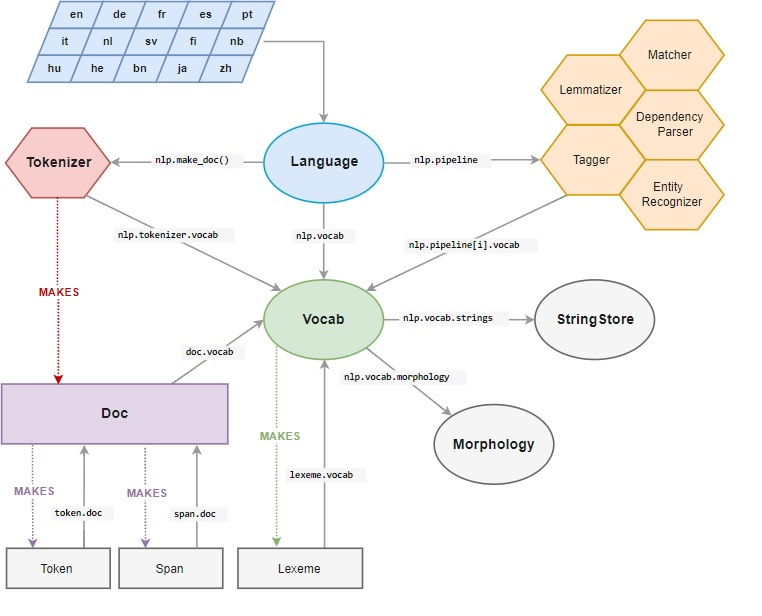
\includegraphics[width=1.2\textwidth]{spacy.jpg}
  \caption{SpaCy Architecture}
  \label{fig:spacy}
 \end{figure}
 
  SpaCy architecture:\newline
 
  Figure \ref{fig:spacy} illustrates a logic schema of SpaCy's internal composition.\newline
  The central data structures in spaCy are the Doc and the Vocab. The Doc object owns the sequence of tokens and all their annotations. The Vocab object owns a set of look-up tables that make common information available across documents. By centralising strings, word vectors and lexical attributes, we avoid storing multiple copies of this data. This saves memory, and ensures there's a single source of truth.\newline

Text annotations are also designed to allow a single source of truth: the Doc object owns the data, and Span and Token are views that point into it. The Doc object is constructed by the Tokenizer, and then modified in place by the components of the pipeline. The Language object coordinates these components. It takes raw text and sends it through the pipeline, returning an annotated document. It also orchestrates training and serialization.
  

  \subsubsection{Data representation}
  \quad Data can be represented as text files or strings. The text contains sentences and paragraphs in English language. Their composition may contain both alpha-numerical characters, symbols and punctuation marks. The data may be sparse, but the logic that dictates linguistic reasoning should be kept in order to obtain relevant information. Random words that make no sense or unnecessary punctuation may lead to bad interpretation and thus, bad results.     

  \subsubsection{Algorithm}
   \begin{enumerate}
  \item  Iterate over space-separated substrings
  \item  Check whether we have an explicitly defined rule for this substring. If we do, use it.
  \item  Otherwise, try to consume a prefix.
  \item  If we consumed a prefix, go back to the beginning of the loop, so that special-cases always get priority.
  \item  If we didn't consume a prefix, try to consume a suffix.
  \item  If we can't consume a prefix or suffix, look for "infixes": stuff like hyphens etc.
  \item Once we can't consume any more of the string, handle it as a single token.
 \end{enumerate}
 
 \subsection{Existing Example}
 \begin{lstlisting}[language=Python]
  doc = nlp(u'Apple is looking at buying U.K. startup for 1 billion')

  for token in doc:
    print(token.text, token.lemma_, token.pos_, token.tag_, token.dep_,
          token.shape_, token.is_alpha, token.is_stop)

 \end{lstlisting}
  Input: String 'Apple is looking at buying U.K. startup for 1 billion'

  The input is turned into a Doc object which holds all the neccessary data (tags) for further processing.
  This "doc" is a tokanized list of the input. After applying the tokenization algorithm previously described, 
  this object is created, where evey word and punctuation mark have a set of definitory tags.

  By creating a for loop, we iterave over each element of the document (i.e., each token) and print out one its tags.
  Example for first element:
   \begin{itemize}
  \item Text: Apple
  \item Lemma: apple
   \item POS: PROPN
  \item TAG: NNP
  \item DEP: nsubj
  \item SHAPE: Xxxxx
 \item ALPHA: True
 \item  STOP: False
 \end{itemize}

  Output: The tags resulted from the tokenization algorithm is printed for each element (word) of the sentence given as a String.

 \subsection{Your own small Example}
 
 \begin{lstlisting}[language=Python]
  import spacy 
  import csv 
  
  nlp = spacy.load('en') 
  doc = nlp('French soldiers march against the German army!') 
  
  for token in doc: 
    print(token.text) 
    
  nationalities = [] 
  nations = [] 
  
  for token in doc.ents: 
  if token.label_ is "NORP": 
      nationalities.append(token) 
  with open('nationalities.csv', 'r', encoding='utf8') as csvfile:
      csvreader = csv.reader(csvfile, delimiter=',') 
      for row in csvreader:
        for nationality in nationalities:
          if str(nationality) == str(row[0]):
            nations.append(str(row[1])) 
            
  print("Nationalities: ") 
  print(nationalities)
  print("Nations:")
  print (nations)
    
\end{lstlisting}

\begin{itemize}
  
  \item My example is given as input a string depicting two combatants of different nationalities. My goal is to extract the nations from the text using spaCy's entry tags. These tags can say whether or not a word depicts a geo-political entity
  or a nationality. However, spaCy offers no way of converting from one to another (i.e., given the nationality German, we cannot infer the nation itself: Germany), and thus, I have chosen a csv file that contains many nation-nationalities relationships
  from GitHub and attached it to the project folder. 
  \item The code creates a Doc object 'doc', prints every token, iterates through them to find nationalities and append them to a list called 'nationalities'. Afterwards, we check every row from the file to see if it fits a nationality from our list. When it
  does, we append the corresponding nation to the 'nations' list. 
  \item The main idea was that, even though we have no GPE (countries) present in the text, we can extract such entities based on the nationalities of the belligerents.
   
\end{itemize}

    
 \subsection{Other issues}
  
  A possible optimization for finding the nation of a given nationality or vice-versa could be loading the whole file in a dictionary type object specific to Python language. This way, access to the needed relationships can be provided much faster. \newline
  
  *This issue was solved.
 
 \section{Proposed problem}
  \subsection{Specification} 
    
  \quad Given a source text which depicts an overview of a historical event, the program must extract the main features of the conflict described in the input. These features may come in the form of:
  \begin{itemize}
      \item Name of the battle
      \item Time of the conflict
      \item Belligerents
      \item Casualties
      \item Winner/loser
      \item Possible aftermath
  \end{itemize}
 
 
  This kind of problem derives from text summarization. The main inspiration came from wikipedia articles which have an abstract that contains such relevant information about historical clashes. \newline
  
  For this problem, we will focus on the Battle of Vienna (Figure \ref{fig:battle}) wikipedia article (mostly its first section) to see if we can precisely pick the relevant data and summarize it. \newline
  Link: https://en.wikipedia.org/wiki/Battle\_of\_Vienna\newline
 
  \begin{figure}
  \centering
  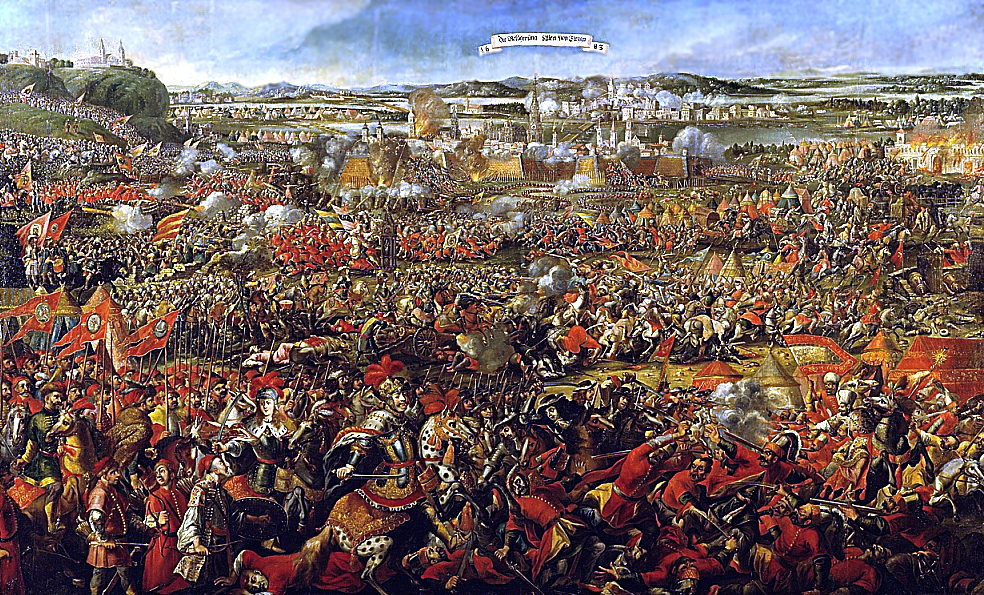
\includegraphics[width=1.0\textwidth]{cover2.jpg}
  \caption{Battle of Vienna 1683}
  \label{fig:battle}
 \end{figure}
 
  For more on text summarization and dependency parsing, please refer to this article and guide:
  \begin{itemize}
      \item A Gentle Introduction to Text Summarization \newline https://machinelearningmastery.com/gentle-introduction-text-summarization
      \item Linguistic Features \newline https://spacy.io/usage/linguistic-features#section-pos-tagging
  \end{itemize}
  
  
  \subsection{Implementation} 
  deadline:  week  12
  
 Implement solution(s) for the proposed problem

  \subsection{Documentation of your solution}
  deadline: week 13
  
  Document your solution: details of data representation, analysis of the results.
  
  \subsubsection{Presentation of your solution}
deadline: week 14

\end{document}          
